\documentclass[a4paper]{article}
\usepackage{pgfplots}
\usepackage{scalefnt} % 文本大小放缩宏包

\begin{document}
{% 调整字体大小
\scalefont{1.2}

% 罗尔定理
\begin{tikzpicture}[line width=1.2pt]
% 画坐标系
\draw[->] (-1.2,0) -- (8.2,0) node[right] {$x$};
\draw[->] (0,-1.2) -- (0,5) node[above] {$y$};
\draw (0, 0) node[below left] {O};

% sin
\draw[domain=1:7.28] plot (\x, {2 + sin((\x - 1.5236) r)});
\draw (4.7, 2.5) node[right] {$f$};

% 切线
\draw (2.07, 3) -- (4.07, 3);

% 辅助线及各种记号
\draw[dashed, color=red] (1, 1.5) -- (7.28, 1.5);
\draw[dashed] (3.09, 3) -- (3.09, 0) node[below] {$\xi$};
\draw[dashed] (1, 1.5) -- (1, 0) node[below] {$a$};
\draw[dashed] (7.28, 1.5) -- (7.28, 0) node[below] {$b$};
\draw[dashed] (1, 1.5) -- (0, 1.5) node[left] {$f(a) = f(b)$};
\end{tikzpicture}

% 拉格朗日中值定理
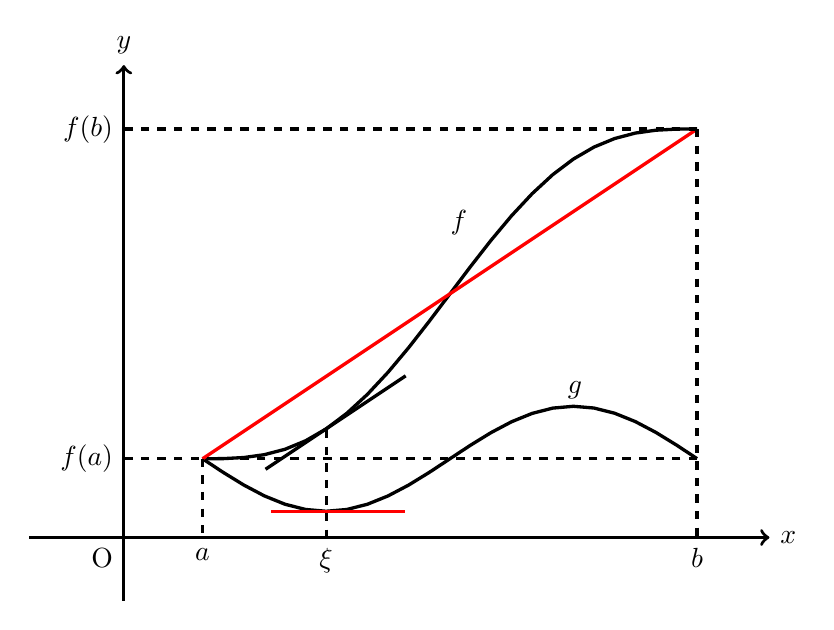
\begin{tikzpicture}[line width=1.2pt]
% 画坐标系
\draw[->] (-1.2,0) -- (8.2,0) node[right] {$x$};
\draw[->] (0,-1.2/1.5) -- (0,9/1.5) node[above] {$y$};
\draw (0, 0) node[below left] {O};

% f = x + sin
\draw[domain=1:7.28] plot (\x, {(1.5 - sin((\x - 1) r) + (\x - 1))/1.5});
\draw (4.5, 6/1.5) node[left] {$f$};

% g = sin
\draw[domain=1:7.28] plot (\x, {(1.5 - sin((\x - 1) r))/1.5});
\draw (5.5, 2.8/1.5) node[right] {$g$};

% 切线
\draw[color=red] (1.87, 0.5/1.5) -- (3.57, 0.5/1.5);
\draw[domain=1.8:3.58] plot (\x, {(\x - 0.5)/1.5});

% 辅助线及各种记号
\draw[color=red] (1, 1.5/1.5) -- (7.28, 7.78/1.5);
\draw[dashed] (2.57, 2.047/1.5) -- (2.57, 0) node[below] {$\xi$};
\draw[dashed] (7.28, 7.78/1.5) -- (7.28, 0) node[below] {$b$};
\draw[dashed] (7.28, 7.78/1.5) -- (0, 7.78/1.5) node[left] {$f(b)$};
\draw[dashed] (1, 1.5/1.5) -- (1, 0) node[below] {$a$};
\draw[dashed] (7.28, 1.5/1.5) -- (0, 1.5/1.5) node[left] {$f(a)$};
\end{tikzpicture}

\begin{tikzpicture}[line width=1.2pt]
% 画坐标系
\draw[->] (-5,0) -- (5,0) node[right] {$x$};
\draw[->] (0,-4) -- (0,4) node[above] {$y$};
\draw (0, 0) node[below left] {$O$};

% f = 1
\draw[domain=0:4] plot (\x, 2);
\draw[fill=white] (0,2) circle (3pt);
% f = -1
\draw[domain=-4:0] plot (\x, -2);

% 辅助线及各种记号
\draw[dashed] (4, 2) -- (4, 0) node[below] {$1$};
\draw[dashed] (-4, -2) -- (-4, 0) node[above] {$-1$};
\end{tikzpicture}

% 零点存在定理
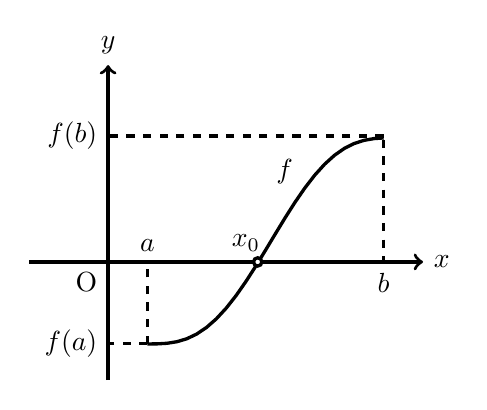
\begin{tikzpicture}[line width=1.2pt, scale = 0.5]
% 画坐标系
\draw[->] (-2,0) -- (8,0) node[right] {$x$};
\draw[->] (0,-3) -- (0,5) node[above] {$y$};
\draw (0, 0) node[below left] {O};

% f = sin x
\draw[domain=1:7] plot (\x, {(-2.5- sin((\x - 1) r) + (\x - 1))/1.2});

% 辅助线及各种记号
\draw[dashed] (1, -2.08) -- (1, 0) node[above] {$a$};
\draw[dashed] (1, -2.08) -- (0, -2.08) node[left] {$f(a)$};
\draw[dashed] (7, 3.1) -- (7, 0) node[below] {$b$};
\draw[dashed] (7, 3.2) -- (0, 3.2) node[left] {$f(b)$};
\draw (4, 2.3) node[right] {$f$};

\draw[fill=white] (3.8,0) circle (3pt);
\draw (3.5, 0) node[above] {$x_0$};
\end{tikzpicture}
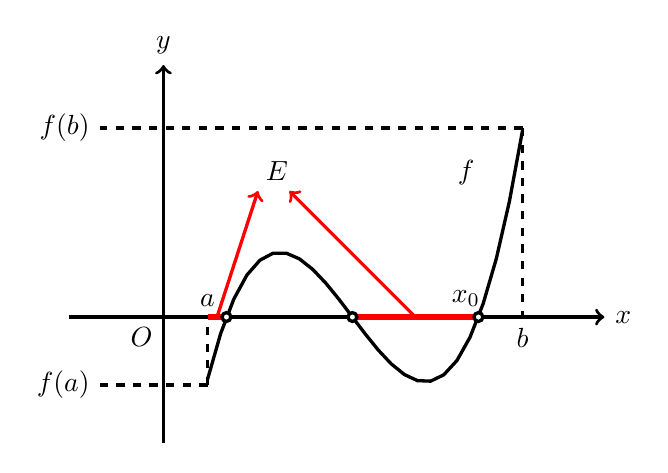
\begin{tikzpicture}[line width=1.2pt, scale = 0.8]
% 画坐标系
\draw[->] (-0.5,0) -- (8,0) node[right] {$x$};
\draw[->] (1,-2) -- (1,4) node[above] {$y$};
\draw (1, 0) node[below left] {$O$};

% f = sin x
\draw[domain=1.7:6.7] plot (\x, {(\x - 2)*(\x - 4)*(\x - 6)/3});

% 辅助线及各种记号
\draw[dashed] (1.7, -1.08) -- (1.7, 0) node[above] {$a$};
\draw[dashed] (1.7, -1.08) -- (0, -1.08) node[left] {$f(a)$};
\draw[dashed] (6.7, 3) -- (6.7, 0) node[below] {$b$};
\draw[dashed] (6.7, 3) -- (0, 3) node[left] {$f(b)$};
\draw (5.5, 2.3) node[right] {$f$};
\draw (6.2, 0.3) node[left] {$x_0$};

\draw[line width=2pt, color = red] (1.7, 0) -- (2, 0);
\draw[line width=2pt, color = red] (4, 0) -- (6, 0);
\draw[fill=white] (2,0) circle (2pt);
\draw[fill=white] (4,0) circle (2pt);
\draw[fill=white] (6,0) circle (2pt);
\draw[->, color = red] (1.85,0) -- (2.5,2);
\draw[->, color = red] (5,0) -- (3,2);
\draw (2.8,2) node[above] {$E$};
\end{tikzpicture}

% 介值定理
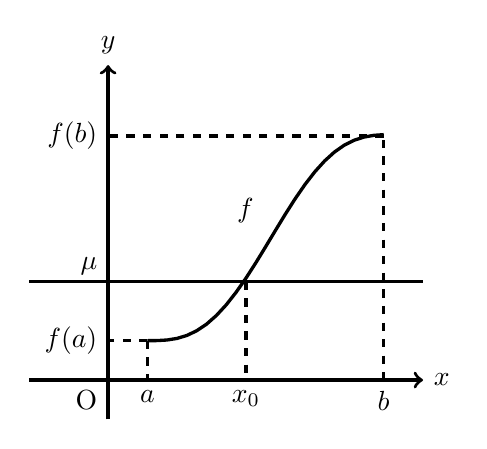
\begin{tikzpicture}[line width=1.2pt, scale = 0.5]
% 画坐标系
\draw[->] (-2,0) -- (8,0) node[right] {$x$};
\draw[->] (0,-1) -- (0,8) node[above] {$y$};
\draw (0, 0) node[below left] {O};

% f = sin x
\draw[domain=1:7] plot (\x, {1 + (0.- sin((\x - 1) r) + (\x - 1))/1.2});
% f = mu
\draw[domain=-2:8] plot (\x, 2.5);

% 辅助线及各种记号
\draw[dashed] (1, 1) -- (1, 0) node[below] {$a$};
\draw[dashed] (1, 1) -- (0, 1) node[left] {$f(a)$};
\draw[dashed] (7, 6.1) -- (7, 0) node[below] {$b$};
\draw[dashed] (7, 6.2) -- (0, 6.2) node[left] {$f(b)$};
\draw (3, 4.3) node[right] {$f$};

\draw[dashed] (3.5, 2.5) -- (3.5, 0) node[below] {$x_0$};
\draw (0, 2.9) node[left] {$\mu$};
\end{tikzpicture}
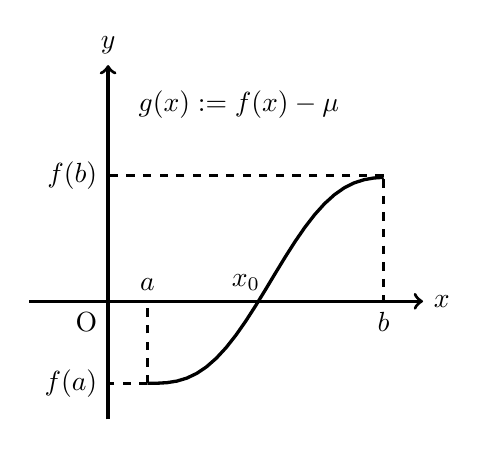
\begin{tikzpicture}[line width=1.2pt, scale = 0.5]
% 画坐标系
\draw[->] (-2,0) -- (8,0) node[right] {$x$};
\draw[->] (0,-3) -- (0,6) node[above] {$y$};
\draw (0, 0) node[below left] {O};

% f = sin x
\draw[domain=1:7] plot (\x, {(-2.5- sin((\x - 1) r) + (\x - 1))/1.2});

% 辅助线及各种记号
\draw[dashed] (1, -2.08) -- (1, 0) node[above] {$a$};
\draw[dashed] (1, -2.08) -- (0, -2.08) node[left] {$f(a)$};
\draw[dashed] (7, 3.1) -- (7, 0) node[below] {$b$};
\draw[dashed] (7, 3.2) -- (0, 3.2) node[left] {$f(b)$};
\draw (0.5, 5) node[right] {$g(x) := f(x) - \mu$};

%        \draw[fill=white] (3.8,0) circle (3pt);
\draw (3.5, 0) node[above] {$x_0$};
\end{tikzpicture}

% 区间
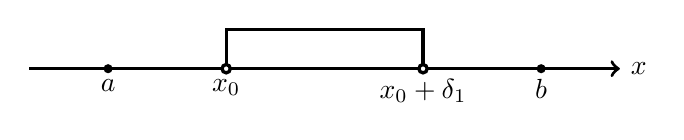
\begin{tikzpicture}[line width=1.2pt, scale = 0.5]
% 画坐标系
\draw[->] (-5,0) -- (10,0) node[right] {$x$};
\draw (-3, 0) node[below] {$a$};
\draw[fill=black] (-3,0) circle (2pt);

\draw (0, 0) node[below] {$x_0$};
\draw (5, 0) node[below] {$x_0 + \delta_1$};
\draw (0,0) -- (0,1) -- (5,1) -- (5,0);
\draw[fill=white] (5,0) circle (3pt);
\draw[fill=white] (0,0) circle (3pt);

\draw (8, 0) node[below] {$b$};
\draw[fill=black] (8,0) circle (2pt);
\end{tikzpicture}

% 区间
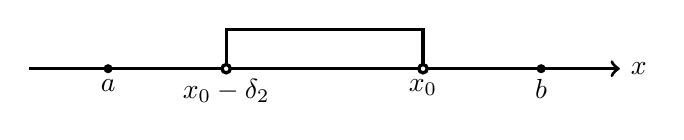
\begin{tikzpicture}[line width=1.2pt, scale = 0.5]
% 画坐标系
\draw[->] (-5,0) -- (10,0) node[right] {$x$};
\draw (-3, 0) node[below] {$a$};
\draw[fill=black] (-3,0) circle (2pt);

\draw (0, 0) node[below] {$x_0-\delta_2$};
\draw (5, 0) node[below] {$x_0$};
\draw (0,0) -- (0,1) -- (5,1) -- (5,0);
\draw[fill=white] (5,0) circle (3pt);
\draw[fill=white] (0,0) circle (3pt);

\draw (8, 0) node[below] {$b$};
\draw[fill=black] (8,0) circle (2pt);
\end{tikzpicture}
}

\begin{center}
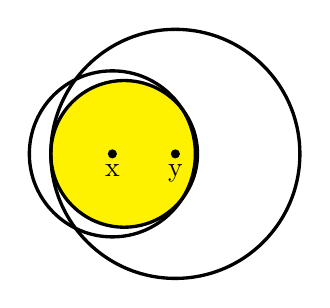
\begin{tikzpicture}[line width=1.2pt]
\draw[fill=yellow] (0.15,0) circle (26.5pt);
\draw (0,0) circle (30pt);
\draw[fill=black] (0,0) circle (1pt);
\draw (0,0) node[below] {x};
\draw (0.8,0) circle (45pt);
\draw[fill=black] (0.8,0) circle (1pt);
\draw (0.8,0) node[below] {y};
\end{tikzpicture}\hspace{0.3cm}
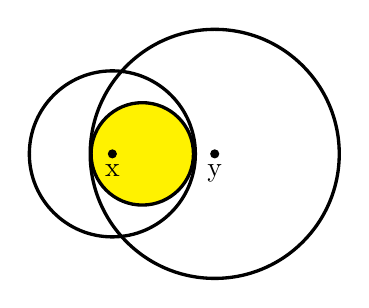
\begin{tikzpicture}[line width=1.2pt]
\draw[fill=yellow] (0.38,0) circle (18.5pt);
\draw (0,0) circle (30pt);
\draw[fill=black] (0,0) circle (1pt);
\draw (0,0) node[below] {x};
\draw (1.3,0) circle (45pt);
\draw[fill=black] (1.3,0) circle (1pt);
\draw (1.3,0) node[below] {y};
\end{tikzpicture}\hspace{0.3cm}
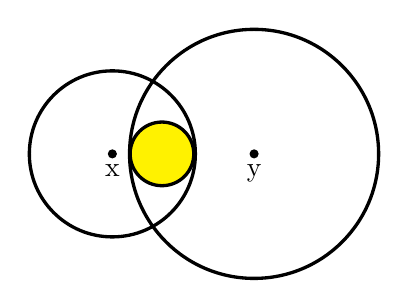
\begin{tikzpicture}[line width=1.2pt]
\draw[fill=yellow] (0.63,0) circle (11.5pt);
\draw (0,0) circle (30pt);
\draw[fill=black] (0,0) circle (1pt);
\draw (0,0) node[below] {x};
\draw (1.8,0) circle (45pt);
\draw[fill=black] (1.8,0) circle (1pt);
\draw (1.8,0) node[below] {y};
\end{tikzpicture}
\end{center}
\end{document}
